\begin{artengenv}{Marek Woszczek}
	{Quantum contextuality as a topological property, and the ontology of potentiality}
	{Quantum contextuality as a topological property, and the ontology of potentiality}
	{Quantum contextuality as a topological property, and the ontology of potentiality}
	{Adam Mickiewicz University in Poznań}
	{Quantum contextuality and its ontological meaning are very controversial issues, and they relate to other problems concerning the foundations of quantum theory. I address this controversy and stress the fact that contextuality is a universal topological property of quantum processes, which conflicts with the basic metaphysical assumption of the definiteness of being. I discuss the consequences of this fact and argue that generic quantum potentiality as a real physical indefiniteness has nothing in common with the classical notions of possibility and counterfactuality, and that also it reverses, in a way, the classical mirror-like relation between actuality and definite possibility.}
	{quantum contextuality, the Bell–Kochen–Specker Theorem, quantum ontology, potentiality, ontic indefiniteness, sheaf theory.}



\lettrine[loversize=0.13,lines=2,lraise=-0.03,nindent=0em,findent=0.2pt]%
{Q}{}uantum contextuality is a~generic property of quantum systems, which is at the same time one of the most contentious issues in the discussions concerning the ontology of quantum theory. There are several reasons for the status of contextuality being so puzzling: some more historical, going back to the early days of quantum mechanics and some more or less hazy discussions around Niels Bohr's philosophical arguments; others purely theoretical, related to the general problems and contemporary analyses concerning the interpretation of the theory.

However, despite these controversies, there is a~growing abundance of experimental tests of contextuality, both state-dependent
%\label{ref:RNDRwqdAOYPjH}(e.g. Liu et al., 2009; Bartosik et al., 2009; Lapkiewicz et al., 2011; Ahrens et al., 2013; Borges et al., 2014; Marques et al., 2014; Singh et al., 2019)
\parencites[e.g.][]{liu_experimental_2009}[][]{liu_experimental_2009}[][]{liu_experimental_2009}[][]{liu_experimental_2009}[][]{liu_experimental_2009}[][]{liu_experimental_2009}[][]{liu_experimental_2009} %
 and state-independent 
%\label{ref:RNDIW1N4VtcJw}(e.g. Amselem et al., 2009; Kirchmair et al., 2009; Zu et al., 2012; Huang et al., 2013; Zhang et al., 2013; D'Ambrosio et al., 2013; Cañas et al., 2014; Dogra, Dorai and Arvind, 2016; Leupold et al., 2018; Qu et al., 2020),
\parencites[e.g.][]{amselem_state-independent_2009}[][]{amselem_state-independent_2009}[][]{amselem_state-independent_2009}[][]{amselem_state-independent_2009}[][]{amselem_state-independent_2009}[][]{amselem_state-independent_2009}[][]{amselem_state-independent_2009}[][]{amselem_state-independent_2009}[][]{amselem_state-independent_2009}[][]{amselem_state-independent_2009}, %
 which have been conducted on many diverse physical systems, including tests using the weak (noninvasive) coupling between systems, as well as recently under the strict no-signaling conditions between successive measurements 
%\label{ref:RNDUMsLsa6XQO}(Xiao et al., 2018).
\parencite[][]{xiao_experimental_2018}. %
 It has also been proposed that contextuality is one of Nature's fundamental physical resources, which has been shown to be crucial in quantum information processing, also in the multiqubit setting 
%\label{ref:RNDSuywzF9i8m}(Raussendorf, 2013; Howard et al., 2014; Bermejo-Vega et al., 2017).
\parencites[][]{raussendorf_contextuality_2013}[][]{raussendorf_contextuality_2013}[][]{raussendorf_contextuality_2013}.%


Nevertheless, there is no single mathematical framework for studying contextuality as a~fundamental physical property, and there also exists a~long tradition of questioning if there is anything nontrivial or mysterious about quantum systems being ‘contextual', with some authors doubting whether it is possible to directly test it in a~lab at all
%\label{ref:RNDksmA5sGk07}(see e.g. Hermens, 2011).
\parencite[see e.g.][]{hermens_problem_2011}. %
 Such a~deep discrepancy between viewpoints is troubling if one seriously acknowledges contextuality to be a~generic property of quantum systems and quantum information processing, since it makes issues related to the ontology of physics even more obscure. After all, if the very physical understanding of quantum contextuality were wholly dependent on some freely chosen philosophical presuppositions, it would be impossible to even define it in a~simple and uncontroversial way, e.g. while preparing and performing experimental tests, which also have their basic tacit ontology of events, measurements and operations. In short, there seems to be a~worrying cleft between recognizing the fundamental nature of contextuality as a~physical resource and its uncertain philosophical interpretation, which seems to be a~matter of taste. I~would like to argue that it is impossible to avoid some free rein in ontological interpretation, but it is not as free as it appears to be, and we should treat contextuality as a~central challenge for quantum ontology.

\section{Quantum contextuality and ontology: more than just another problem}
In general terms, contextuality is the impossibility of a~consistent, global assigning of the pre-existing $\{0,1\}${}-values (i.e. binary definite properties) to all possible synchronic physical observables on a~quantum system for $\mathit{dim}>2$, which is a~serious deviation from the classical-mechanical case where such assignments are in principle always possible. In a~more physical framing, this means that there is an unavoidable contradiction between such a~pre-assignment of values and the intuitive expectation that the measurement outcome does not depend on other comeasurable observables. Mathematically, this is expressed by the celebrated (Bell–)Kochen–Specker Theorem (henceforth, BKS) proved in 1966-1967 for finite sets of observables
%\label{ref:RNDVqwfzQKSNg}(Kochen and Specker, 1967),
\parencite[][]{kochen_problem_1967}, %
 which is a~particular consequence of a~theorem with fundamental importance for quantum mechanics, namely the Gleason Theorem 
%\label{ref:RNDKoGlU23Gip}(Gleason, 1957).
\parencite[][]{gleason_measures_1957}.%


A~precursor of this result was Specker's short but ingenious paper
%\label{ref:RNDBJIgaXwusZ}(Specker, 1960),
\parencite[][]{specker_logik_1960}, %
 in which he studied the deep logical structure of the co-decidability of propositions concerning any quantum-mechanical system and their embedding into Boolean lattices while preserving the operations of negation, conjunction and disjunction, and answered by ‘an elementary geometrical argument' in negative the hope of having the $\{0,1\}${}-valuations for those propositions. In fact, both Specker's motivation and result had conspicuous metaphysical overtones, since their main, innocent-looking target was the idea of the scholastic or Leibnizian-like ‘Absolute Observer', which is just a~fancy name for the consistent structure of the Boolean valuations defining the determinate, global actual state of a~physical universe characterized by an ordered set of propositions. Thus, Specker's answer is quite plain: such a~Leibnizian omniscient spectator of the state of affairs, or, equivalently, such a~globally determinate actual state (‘reality'), cannot exist without contradiction. Then, one decade after Gleason's formal result, John S. Bell 
%\label{ref:RNDK0nlVH336x}(Bell, 1966)
\parencite[][]{bell_problem_1966} %
 addressed the problem in the framework of the hidden variable deterministic models, i.e. always possessing the dispersion-free states, and he correctly observed that such models cannot be constructed if they are expected to be entirely noncontextual since the additivity of the expectation values for comeasurable observables cannot hold. The significance of these purely formal results is today quite clear, yet their ontological meaning is not. In what follows, I~shall exclusively focus on this purely metaphysical side of the problem, thus ignoring the semantic or epistemological aspects, since the main point of interest here is to gauge the prospects for a~realistic ontology of physical (quantum) potentiality \textit{in mundo}.

Before we proceed to the topological and physical meaning of contextuality, let us straighten out why the whole issue is so serious from the purely philosophical point of view. The question is, after all, what does the ‘impossibility of the pre-existing $\{0,1\}${}-values of observables' (‘impossibility of binary definite valuations') mean?

There is a~deep philosophical controversy lurking behind this question, since the central problem at issue here is, as far as we try to faithfully construe the formal structure of quantum theory, that of \textit{physical definiteness} (henceforth, \textbf{D}) and \textit{objective reality or pre-existence} (\textbf{OR}). In fact, from the ontological point of view, \textbf{D} and \textbf{OR} are closely interlinked, as the core ingredients organizing basic metaphysical arguments and constructions, since the fundamental assumption of the Western realist metaphysics after Parmenides, Plato and Aristotle, also inherited by post-ancient physics, and mechanics in particular, is:

[\textbf{DOR}]

Being real (Greek \textgreek{>'on}) = being definite (\textgreek{tod'i ti}) = being a~part of a~determinate, consistent whole (\textgreek{t`o <'olon}) or a~logical complemented system (\textgreek{l'ogos}).

The precondition is that an objective being\footnote{Not an image or subjective representation of a~being, which may be deficient, uncertain, inaccurate or fuzzy. } exists and is comprehensible only in a~determinate whole, in which maximal mutual distinguishability and definite exclusion (complementation) relations between all its constituent elements are always guaranteed. \textbf{DOR} is the guiding classical ontological intuition concerning, for example, states or elements of some definite world, actual or possible, which is why anything which would deviate from it has been taken to be both nonexisitent and incomprehensible, irrational in the strong sense of the term (alogical, in Greek \textgreek{>al'ogos}).

For example, in his \textit{Republic} Plato is explicit that ‘what fully exists is also entirely intelligible, and what does not exist is also unintelligible' (\textit{Rep}. 477a3-4).\footnote{Here and thereafter all translations from the sources are mine. For the sake of clarity, I~take Plato's \textgreek{e>'idh}} from \textit{Sophist} 259e and \textgreek{m'oria} from \textit{Parmenides} 158c-d as meaning ‘elements' (of some complete system). And in the dialogue \textit{Sophist} it is emphatically stated that intelligibility is possible only in the whole system of propositions, i.e. \textit{logos}, which forms a~complete system of definite elements\footnote{In the pre-classical Greek, the meaning of \textit{logos} is just a~gathering or putting together of some discrete elements.} and their exclusion relations, beyond which nothing can be comprehended at all: ‘to separate each thing from everything else is a~total destruction of the logos, for what makes logos possible is interdependence between all elements' (\textit{Soph}. 259e4-6). According to this way of thinking, every element in itself has no definite nature in separation, and only when taken as a~part of such a~complete system of logical relations (\textit{logoi}) can it be regarded as some real being: ‘whenever each element becomes a~single element, it has a~limit in relation to any other element and to the whole, and that whole also has it in relation to all its parts' (\textit{Parm}. 158c7-d2). That is why the metaphysical status of Aristotle's prime matter (\textgreek{pr'wth <'ulh}) as an ultimate \textit{potentia} or an utterly formless ‘bare stuff' is so questionable and vague, since something which is totally indefinite, i.e. falls outside the system of logical categories of predication, cannot exist \textit{per se} as reality, and cannot be invoked as some efficient potentiality taken as a~self-standing substrate of what actually exists
%\label{ref:RNDSQhdAeM1xW}(see e.g. Charlton, 1992).
\parencite[see e.g.][]{aristoteles_appendix_1992}. %
 In fact, the ‘prime matter', in line with \textbf{DOR}, is rather non-being.

Most modern philosophical discussions concerning indeterminacy or fuzziness (taken to be equivalent) have been focused on logical, semantic-representational and purely epistemological aspects related to vague predicates and epistemic or pragmatic uncertainty, while the metaphysics of ontic indefiniteness \textit{in mundo}, especially in the foundations of physics, has been given, due to the appeal of \textbf{DOR} and troublesome maladies such as the Sorites Paradox\footnote{See e.g.
%\label{ref:RNDUv2K2hCRet}(Dummett, 1975)
\parencite[][]{dummett_wangs_1975} %
 for a~classic argument of this kind against fuzzy predicates and indeterminacy as unacceptable and unintelligible, that is, pathological for any coherent system. Assuming a~semantic analogue of \textbf{DOR} and the classical logic, Dummett famously claimed, in a~somewhat Platonic vein, that phenomenal properties as commonly conceived cannot be real. The same could apply to all versions of the Sorites Paradox.}, only little attention. In fact, it is common after Russell to assume that indefiniteness itself and the failure of the principle of the excluded middle both signal merely epistemic vagueness or subjective ‘indecision', and cannot be accepted as an essential ingredient of consistent, fully realistic (i.e., proclaiming \textbf{OR}) metaphysics and physics. In this sense, \textbf{D} makes up a~necessary, though not sufficient, condition of classical realism as encapsulated in David Lewis's stringent dictum: ‘The only intelligible account of vagueness locates it in our thought and language. […] Vagueness is semantic indecision' 
%\label{ref:RNDI8CpmKl7ES}(Lewis, 1986, p.212).
\parencite[][p.212]{lewis_plurality_1986}. %
 Contemporary metaphysical approaches which posit some ontic indeterminacy together with \textbf{OR} mostly do not introduce it at the basic level of the constituent identity-laden worldly entities, thus they are compatible with standard mereology 
%\label{ref:RNDx7NVrNYk61}(cf. e.g. Morreau, 2002).
\parencite[cf. e.g.][]{morreau_what_2002}. %
 Even more elaborate theories working in the modal framework 
%\label{ref:RNDhykWiKmjzA}(e.g. Akiba, 2004; Barnes and Williams, 2011)
\parencites[e.g.][]{akiba_vagueness_2004}[][]{akiba_vagueness_2004} %
 admit primitive ontic indeterminacy, but they often uphold bivalent classical logic and semantics as their firm backbone. In such cases, \textbf{DOR} operates undisturbed at the higher level of possible worlds being complete (maximal) and fully determinate systems, and it is just objectively indefinite which of them is actualized in time.

Thus, in essence, the Western ontological and physical paradigm based on \textbf{DOR} assumes that being something means being a~certain determinate entity (e.g. ‘this thing' or ‘this fact'), which is logically defined in terms of multiple relations, in particular the exclusion negation (complementation)\footnote{The ontological nature of negation is at the very centre of the dialogue, cf. \textit{Soph}. 258a-c. It was Proclus in the 5\textsuperscript{th} century AD who in his commentary on Plato took it to extremes, saying that ‘negations are causes (\textgreek{a>'itiai}) of affirmations' (\textit{In Parm}., VI, 1075, 18-19; cf. Proclus, 1992, p. 428).} , in a~total propositional system which does not license any first-order vague predicates corresponding to real indefinite properties, including dispositions. Perhaps the most mature and radical fruit of this tradition in early modern philosophy is Leibniz's masterly binary ‘universal algebra of concepts' from his \textit{Generales inquisitiones}… (1686)\footnote{This ‘universal calculus' of definite concepts is just Boolean algebra before Boole
%\label{ref:RNDqIBDi52U34}(Lenzen, 1984; Malink and Vasudevan, 2016),
\parencites[][]{lenzen_leibniz_1984}[][]{lenzen_leibniz_1984}, %
 equipped with identity, containment, conjunction and negation.} and the related full-fledged essentialist ontology of possible worlds as global logical systems composed of completely definite, indivisible individuals characterized by intrinsic states 
%\label{ref:RNDYvIZoCgpBi}(see e.g. Bella, 2005).
\parencite[see e.g.][]{bella_science_2005}. %
 Here, reality itself is thoroughly definite, and there is an ideal ‘Absolute Observer' associated with such a~complete system. Leibniz offers a~clear picture of every definite universe-system as governed “by laws of the general order (\textit{Loi de l'ordre general}) of this possible universe to which they are appropriate and whose concept they determine, as they do also the concepts of all the individual substances which compose that particular universe'' 
%\label{ref:RNDidO7Uuu15K}(Leibniz in a~letter to A. Arnauld, 14 July 1686; Leibniz, 2009, p.73).
\parencites[][]{}[][p.73]{leibniz_samtliche_2009}. %
 The Leibnizian panoptical ‘Absolute Observer' of the world-system is exactly the omniscient God from Specker's 1960 paper, who might check in advance by logical calculation the $\{0,1\}${}-value of any proposition about the future contingent value of any possible physical observable. Note that here the ontological relation between the possible and the actual is always mirror-like: the systemic rules of construction and the global $\{0,1\}${}-determinacy of worlds are the same all along.

\textbf{DOR} seems to be extremely important for physics, and science in general, since it is a~necessary foundation of the Principle of Sufficient Reason (PSR), which states that for every state or fact \textit{F} of a~world, there is a~definite reason why \textit{F} is the case, or, in Spinoza's famous phrasing, ‘\textit{si nulla detur determinata causa, impossibile est, ut effectus sequatur}'.\footnote{‘If there is no determinate cause, it is impossible for any effect to follow'
%\label{ref:RNDldbrmWxg27}(Spinoza, \textit{Ethics}, I, Ax. III; Spinoza, 1977, p.6).
\parencites[][]{}[][p.6]{spinoza_ethik_1977}.%
} In other words, whatever contingent physical fact (actual value of some observable) is taken into account, there must be a~definite ground for its coming to be, e.g. some other \textit{definite state} and its evolution. PSR can be transferred to the indeterministic setting in ontology and we can accept a~generalized probabilistic explanation for any \textit{F}, e.g. by use of the category of disposition or propensity, but in order to have a~consistent picture of reality one needs an agreement concerning both (i) what a~definite fact \textit{F} is (\textit{objectivity of actual states}), and (ii) what a~definite disposition for coming to be of \textit{F} is (\textit{objectivity of determinate possibility}). In order to have (ii) being concordant with \textbf{DOR}, it is necessary to have a~complete basis of all determinate possible (Boolean) states of affairs, which can then carry the pre-assigned values of the (Boolean-Kolmogorovian) probability measure construed as representing the complete ontic dispositions pertaining to an actual system. Let us call such possible states the classical (or Leibnizian) possibilities. If either (i) or (ii) does not work, or if neither works, then the whole ontological framework falls through, along with PSR as its foundation. In such cases, strong ontic indefiniteness seems to spoil the very idea of OR.

Another consequence of assuming \textbf{DOR} in physics is also Einstein–Podolsky–Rosen's
%\label{ref:RNDhUWbS00e2f}(1935)
\parencite*[][]{bohr_can_1935} %
 famous definition of the ‘elements of reality' in terms of what can be predicted (\textit{via} physical laws or computability) with certainty: being real means being actual and fully definite, which always requires, at least in principle, globally consistent $\{0, 1\}$-valuations for separate states of affairs occuring at any spatiotemporal location. Einstein called it \textit{So-Sein}, ‘being-thus', and made it the essence of his principle of separability. The point is that \textbf{DOR} is so prevalent and habitual that EPR physical reasoning seems inescapable under the threat of contradiction: if the world is composed of determinate facts \textit{F}, and is consistent as the reality, there has to be a~\textit{global} $\{0, 1\}$-valuation on \textit{all possible} synchronic physical observables on all \textit{actual} physical systems, whatever their interactions are. That is in essence what reality is. Niels Bohr's quick answer to the EPR paper 
%\label{ref:RND2ibbxdZvQm}(Bohr, 1935)
\parencite[][]{bohr_can_1935} %
 rejected that assumption, hence it also dropped \textbf{DOR}, but did so by relying on epistemological considerations and the classical notion of the ‘experimental arrangement' and ‘eventuality' without any clear ontology, which led to the obscurity of his \textit{quasi}-Kantian phrase which referred to contextuality as ‘an influence on the very conditions which define the possible type of predictions regarding the future behaviour of the system'
%\label{ref:RNDNNPEdtL5su}(Bohr, 1935, p.700).
\parencite[][p.700]{bohr_can_1935}.%


Perhaps this is also the main reason why John S. Bell
%\label{ref:RNDlZSt8hreTV}(1981, pp.58–59)
\parencite*[][pp.58–59]{bell_bertlmanns_1981} %
 wrote that for him Bohr's reply, which relied on the complete ‘freedom of handling the measuring instruments', is incomprehensible, while the EPR clear ontological standpoint concerning the ‘nature of reality', which respects \textbf{DOR}, is not. Bell was perfectly right when he stressed that what is at stake is not just the old problem of determinism or some particular correlations \textit{per se}, but rather, in line with Bohr, the commonsense definition of reality\footnote{Bell 
%\label{ref:RNDS8tRgzEZ6W}(1981, pp.45–46)
\parencite*[][pp.45–46]{bell_bertlmanns_1981} %
 humorously wrote that Einstein, Podolsky and Rosen ‘were with the man in the street in this business'.} and physical systems having some pre-assigned definite properties that are locally detected (measured). And it was Bell himself who constructed the first proof of the state-dependent contextuality for quantum compound systems dissociated in space 
%\label{ref:RNDZkx7ISVIKp}(Bell, 1964),
\parencite[][]{bell_einstein-podolsky-rosen_1964}, %
 before it was fully realized that the resulting nonlocality is mathematically just a~particular instance of the more general contextuality 
%\label{ref:RNDkNbAXdAYEQ}(e.g. Horodecki et al., 2015; Acín et al., 2015).
\parencites[e.g.][]{horodecki_axiomatic_2015}[][]{horodecki_axiomatic_2015}.%
\footnote{The nonexistence of joint probabilites for quantum systems does \textit{not} depend on any distance in spacetime. Spatial separation between subsystems and the nonlocal correlations only make conspicuous the generic nonclassicality of this contextuality. One may call it \textit{general nonseparability}, also in the case of non-composite systems.} It seems clear that the latter is indeed, with respect to \textbf{DOR} and the impossibility of consistent $\{0,1\}$-valuations 
%\label{ref:RNDORVpIrvk7D}(Bohr, 1935, p.699),
\parencite[][p.699]{bohr_can_1935}, %
 a~severe ontological problem, of course to the extent that one wants to have some explicit realistic ontology at all.

\section{Ontic quantum contextuality as a~topological property}
Let us define formally what is so curious about physical contextuality and why such a~basic and apparently innocuous assumption as \textbf{DOR} is questionable precisely on ontological grounds, including the notion of classical possibility. In order to make fully explicit the topological difference between the classical and quantum structures of observables, as well as between the corresponding notions of ‘state', we adopt here a~theory-dependent formulation of contextuality, in contrast to e.g. the general theory-independent framework proposed by Abramsky \& Brandenburger
%\label{ref:RNDcEB309PBNK}(2011)
\parencite*[][]{abramsky_sheaf-theoretic_2011} %
 in terms of sheafs over the space of empirical measurement scenarios.

Let $\mathcal{S}(\bm{B})$ be a~topological Stone space of the Boolean algebra $\bm{B}$ of propositions about the synchronic physical properties of some classical system $O$, which means that $\mathcal{S}$ effectively encodes the relevant physics of $O$ (whatever it is: gravitational, electromagnetic, or other). This is quite obvious since any pure mechanical state $\psi $ of $O$ automatically selects an ultrafilter in $\bm{B}$, and the field of all ultrafilters in $\bm{B}$ is isomorphic to $\bm{B}$~as its dual topological Stone space $\mathcal{S}(\bm{B})$ due to the Stone representation theorem. And let $\bm{\mathcal{T}}_{\mathcal{S}} = (\mathcal{T}, \pi, \mathcal{S})$ be the constant Boolean sheaf over the state space $\mathcal{S}$, that is, every stalk $\mathcal{T}_{S}$ is fixed as $\mathcal{T}_{S} = \pi_{-1}(\{s\}) = \bm{2} \equiv \{0,1\}$, $s{\in}\mathcal{S}$, with the projection $\pi:\mathcal{T}\to\mathcal{S}$ as a~local homeomorphism from the étalé space $\mathcal{T}$. Local sections of the sheaf $\bm{\mathcal{T}}_{\mathcal{S}}$ over the proper subsets $S{\subset}\mathcal{S}$ are continuous maps $\sigma :S\to \mathbf{2}$, where $\pi \circ \sigma = id_S$, which gives the values $\sigma(S)$ of the sheaf. By definition, a~section is global when $S = \mathcal{S}$, and then every $\sigma $ is just a~restriction of the latter
%\label{ref:RNDi91cKUjmUF}(Mac Lane and Moerdijk, 1992, chap.II; Knoebel, 2012).
\parencites[][chap.II]{mac_lane_sheaves_1992}[][]{mac_lane_sheaves_1992}.%


The fundamental fact about the classical-mechanical spaces of pure states $\psi $ of any $O$ is that one can always have global sections of $\bm{\mathcal{T}}_{\mathcal{S}}$, and the full algebra $\bm{\Gamma}_{\mathcal{S}}(\mathcal{T})$ of those sections is just isomorphic to $\bm{B}$, which is a~constructive backbone of classical mechanics. In the classical world we can always locally glue information into a~single coherent picture of the actual properties of $O$ by consistent Boolean valuations, that is, it is possible to consistently extend any local $\sigma$ for $S=\mathcal{S}$: the global, i.e. unrestricted, sections over $\mathcal{S}(\bm{B})$ \textit{do always exist} (Fig. \ref{woszczek-fig1}). One can thus say that the logic of constant $\{0,1\}$-valuations is ‘flat' or well-behaved, or, that the corresponding sheaf is trivial, which makes the question of what counts as reality quite unproblematic and the whole scaffolding of the physical reference frames to be of purely epistemic character.

\begin{figure}
\centering
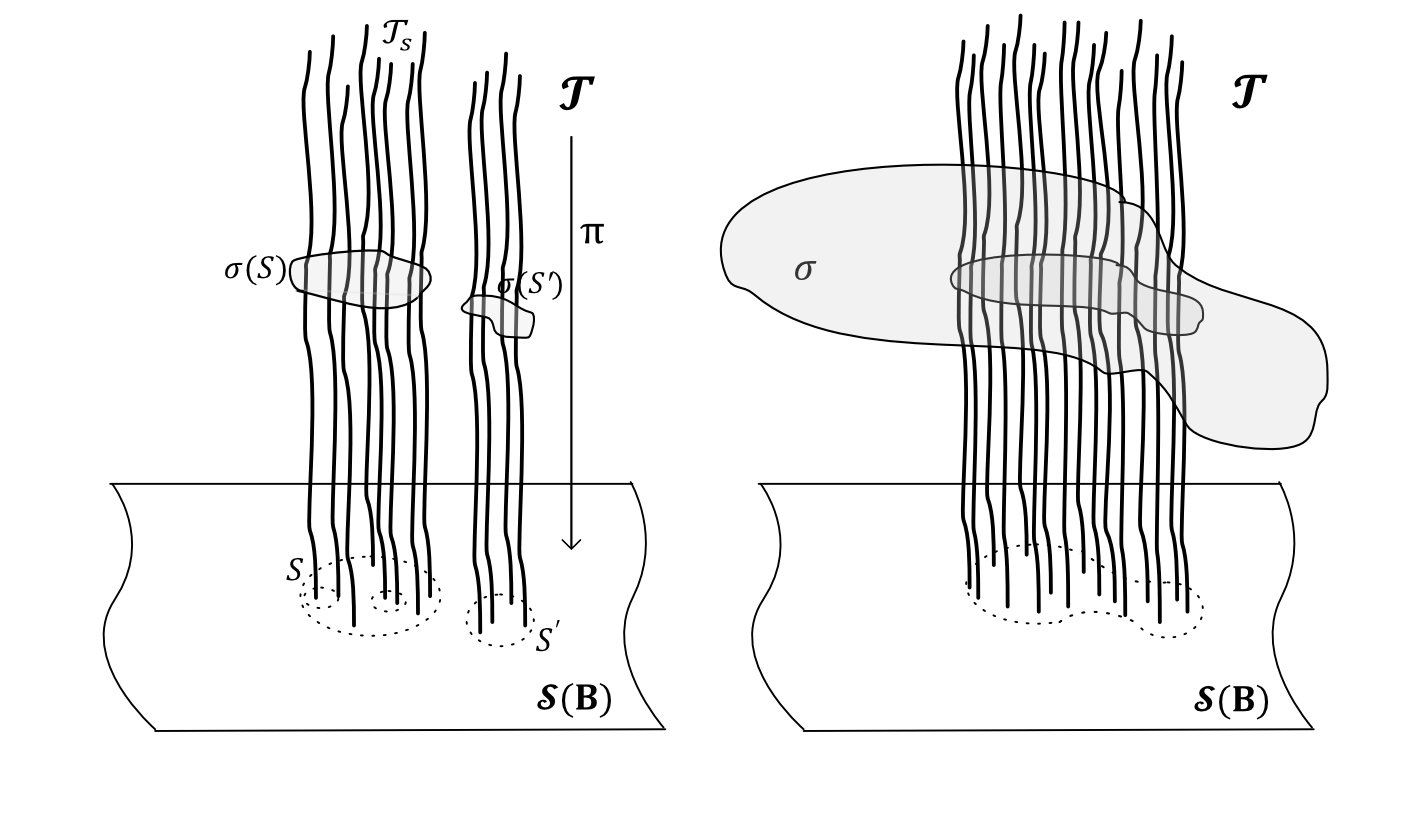
\includegraphics[width=.7\textwidth]{ART_Woszczek/Woszczek.jpg}
\caption{}\label{woszczek-fig1}
\end{figure}

In fact, what is of crucial importance is that, due to the existence of ultrafilters, the very notion of physical state as a~catalogue of the actual properties of $O$~becomes straightforward; each physical system has its own Einsteinian ‘being-thus', and, moreover, there is no difficulty in extending this notion to the whole universe (world-$\Psi$) taken as a~mechanical system of $O$'s. This means that any ontic contextuality of states is absent, and there is only one global ‘context' of coexisting properties without restrictions, which is encapsulated by the metaphysical catchword ‘Absolute (panoptical) Observer'.

Note that since the ultrafilters on $\bm{B}$ simultaneously generate the full Boolean algebra of all the global sections of $\bm{\mathcal{T}}_{\mathcal{S}}$, that is $\bm{B\cong\Gamma}_{\mathcal{S}}(\mathcal{T})$, one gets the algebra of the classically possible (Leibnizian) mechanical worlds, which is already built from the very beginning into the unitary logical framework. The curious ‘mirroring' feature of the latter is that it is \textit{exactly the same logic} which governs the domains of the possible and the actual, hence there seems to be nothing special about possibility \textit{per se} -- in fact, it is difficult to comprehend why the actual would be ontically distinguished as ‘fully existing'. That is why thinkers like Leibniz needed a~ladder of additional metaphysical constraints as rules of the world selection, or foreknowing God's one-moment choice, while in the classical deterministic cosmology there is always the problem of the extremely improbable boundary conditions and the unpleasant cosmological fine-tuning of the initial (or final) world- $\Psi $ as a~bare fact. It looks like the domain of possibility was fully modelled upon the domain of actuality, and the probabilities for the latter could be consistently pre-assigned only after some complete universe of logically possible states of affairs, i.e. the full Boolean algebra $\bm{\Gamma}_{\mathcal{S}}(\mathcal{T})$, is fixed (that is how the probability of ‘improbable boundary conditions' is assessed).

Even if one prefers the indeterministic ontology and objective (noncontextual) dispositions or propensities, like e.g. Karl Popper
%\label{ref:RNDlNn26X3DSB}(1967),
\parencite*[][]{popper_quantum_1967}, %
 it is tacitly assumed that there is no way beyond the Kolmogorovian measure based on $\bm{\Gamma}$. The reason behind this premise is not just PSR and the requirement of concordance between (i) and (ii), it lies much deeper, in ontological \textbf{DOR}: one needs a~complete basis of definite (Boolean) elements for the probabilistic measure, and then (\textit{i}) and (\textit{ii}) can be handled in a~unitary manner. In the end, there is no way out of the Boolean universe here. The logical state structure $\bm{\Gamma}_{\mathcal{S}}(\mathcal{T})$ in physics is thus a~full realization of the paradigmatic ontological intuition, since being means being definite \textit{and} being a~part of some fully determinate, consistent whole, which brings forth, as a~sort of a~byproduct, the idea of panopticality or a~detached observer. One may sum this up by saying that classical ontology favours the actual and the definite, paying the price of making the potentiality a~mirror image or an expanded shadow of the actual.

In the quantum regime, the rules of the game change drastically. A~lattice of propositions about the properties of a~quantum system $O$ (which may also be multipartite) forms an orthomodular $\sigma $-orthoposet $\bm{\mathfrak{L}}(\mathcal{H})$, being isomorphic with the lattice of closed subspaces of the complex Hilbert space $\mathcal{H}$ associated with $O$, which is complete if it is ordered by inclusion (for simplicity we limit ourselves to cases when $\mathcal{H}$ can be constructed at all, but it can be generalized to all types of $W^{\ast}$-algebras of observables, see
%\label{ref:RNDYwzuYMFRzx}(Döring, 2005)
\parencite[][]{doring_kochenspecker_2005}%
). The sheaf-theoretic construction for quantum observables may be achieved in general as follows. Let a~topological space $\mathcal{L}_{\bm{\mathfrak{L}}(\mathcal{H})}$ be a~family of all Boolean (commutative) subalgebras $L$ of $\bm{\mathfrak{L}}(\mathcal{H})$ ordered by inclusion ${\subseteq}$, and let us have a~required Boolean homomorphism (the Kochen–Specker valuation) $h:L\to \bm{2}$ for any $L_i{\in}\mathcal{L}_{\bm{\mathfrak{L}}(\mathcal{H})}$. We can define the partial ordering $\leq$ for pairs $(L_i,h_i)$, given by: $(L_1,h_1){\leq}\left(L_2,h_2\right)$ iff $L_1{\subseteq}L_2$ and $\left.h_1=h_2\right|L_1$, associated with the respective topology of $\mathcal{L}_{\bm{\mathfrak{L}}(\mathcal{H})}$. Every Boolean subalgebra $L_i$ in $\mathcal{L}_{\bm{\mathfrak{L}}(\mathcal{H})}$ belongs to some maximal Boolean subalgebra (a maximal quantum observable), which forms a~(quasi-) classical \textit{context} $\bm{\mathfrak{M}}$.

Now the \textit{quantum spectral sheaf} (over the base space of quantum observables or spectral algebras), the closest analogue of the classical $\bm{\mathcal{T}}_{\mathcal{S}}$ we get, is a~triple $\bm{\Phi}_\mathcal{L} = (\Phi, \pi, \mathcal{L}_{\bm{\mathfrak{L}}(\mathcal{H})})$, with $\Phi_{L_i}=(L_i,h_i:L_i{\in}\mathcal{L}_{\bm{\mathfrak{L}}(\mathcal{H})})$ and a~projection as a~surjective local homeomorphism (étale map) $\pi :\Phi \to \text{[27F6?]}$ from the sheaf space $\Phi $. A~continuous local section (of the projection $\pi$) over some subset $M \in \mathcal{L}_{\bm{\mathfrak{L}}(\mathcal{H})}$ is a~map $\sigma: M \to \Psi$, $\pi \circ \sigma =\mathit{id}_M$, and the images of local sections naturally induce the topology for the whole étalé space $\Phi$. That is so because for every $L_i \subset M$ we obviously get $\{0,1\}$-values of the sheaf, $\sigma (L_i)=(L_i,h_i)$, with the proper restriction condition: $\sigma (L_1)=(\left.L_2,h\right|L_1)$ for every $L_1\subseteq L_2$, which always guarantees the local compatibility of sections as a~crucial fact about the quantum observable values. Due to Gleason's no-disturbance principle for $\mathcal{L}_{\bm{\mathfrak{L}}(\mathcal{H})}$, the probability for obtaining some value cannot depend on a~valuation of some other compatible observable, which gives the properly behaving, i.e. additivity satisfying, probabilities for $\bm{\mathfrak{M}}$'s
%\label{ref:RNDyf3gAnFNxU}(Gleason, 1957).
\parencite[][]{gleason_measures_1957}.%
\footnote{In the operational framework, one might call this central property the ‘noncontextuality of projective measurements'. However, it should be remembered that it is a~purely algebraic feature of the whole quantum structure, and not just the statistical characteristics of particular sets of measurement outcomes.} Hence the latter define subclassical ‘patches' within the full quantum $\bm{\mathfrak{L}}(\mathcal{H})$, and the essence of the generic quantum complementarity is that it is not possible to have the full $\{0,1\}$-valuations (i.e. the Kochen–Specker states) over two different $\bm{\mathfrak{M}}$'s at the same time.\footnote{See e.g. 
%\label{ref:RNDZs9dzkK0Uy}(Heunen, Landsman and Spitters, 2012)
\parencite[][]{heunen_bohrification_2012} %
 for a~purely operator-algebraic account of quantum complementarity, and 
%\label{ref:RNDUOLqvF5lBt}(Heunen, 2012)
\parencite[][]{heunen_bohrification_2012} %
 for a~general categorical approach in terms of dagger monoidal kernel categories.}

The (Bell–)Kochen–Specker Theorem in the sheaf-theoretic formulation simply says that if a~Hilbert space $\mathcal{H}$, representing the physics of a~system $O$, is of $\mathit{dim} > 2$, then the spectral sheaf $\bm{\Phi}_{\mathcal{L}}$ on $\mathcal{L}_{\bm{\mathfrak{L}}(\mathcal{H})}$ has \textit{no global sections}. Thus, we have a~strong topological obstruction, which makes the unrestricted extending of local $\sigma$ impossible if the global consistency of valuations $\sigma (L)$, as in the case of $\sigma (S)$ for $\mathcal{T}_{\mathcal{S}}$, has to be preserved (ultimately, that is what the objectivity of states (i) and the EPR intuition about the definite ‘elements of reality' do unconditionally demand). A~global Boolean ‘context' for mechanics does not exist, and only single local contexts $\bm{\mathfrak{M}}$, as defined by quantum spectral algebras, can be regarded as being definite, hence the whole idea of synchronic $\{0,1\}$-properties, objectively preexisiting and pertaining to $O$ as ‘states', gets into fatal trouble.

In consequence, what is actual, i.e. a~definite fact F~from (i), is only a~\textit{random local section} $\sigma (L)$ of $\pi$ in a~particular definite $\bm{\mathfrak{M}}$, and that physically relativizes the valuation $h$ itself, which is a~contingent relation of $O$ to some exosystem $O'$ that induces the particular $\bm{\mathfrak{M}}$.\footnote{Due to the standard minimal interpretation of the situation, quantum mechanics cannot be -- and is not -- metaphysically realist in the \textit{classical} meaning of the term, which is quite obvious. But the stronger claim that it cannot be realist at all (in any acceptable sense) is premature and overly dependent on the classical metaphysical framework of actuality and its ‘mirroring' possibility, that is $\bm{B\cong\Gamma}_{\mathcal{S}}(\mathcal{T})$. In fact, it rests on the acceptance of \textbf{D} as a~putative necessary condition of realism \textit{per se}.} Quantum mechanics simply lacks the constructive backbone of its classical predecessor. Before I~discuss what this means for any ontological account of potentiality, it is important to indicate why this topological obstruction has nothing to do with the classical epistemic contextuality and should be physically dealt with as a~fully ontic property. These arguments are thus based on strictly physical, including experimental, considerations, being at least relatively independent from contestable metaphysical presuppositions, and they range from quantum-informational to thermodynamical aspects. In essence, $\bm{\Phi}_L$ induces the totally nonclassical structure of \textit{physical} probability and entropy, and that only in turn effectively restrains ontologies with definite states or dispositions modelled after $\bm{\Gamma}_{\mathcal{S}}(\mathcal{T})$ (I shall go back to the latter point in the next section).

Firstly, the topological obstruction on $\bm{\Phi}_L$ gives rise to the entirely novel physics of information processing in Nature, the objective (non-epistemic) quantum regime, which has nothing to do with human labs and disturbance-producing experiments. At the level of the latter, due to the contextuality or algebraic ‘locality' of $\sigma (L)$, it is impossible to perfectly distinguish some unknown pure nonorthogonal quantum states, and thus to determine in one shot an unknown state on a~single copy, however weak the conceivable measurement is
%\label{ref:RNDuquyajTMxC}(D'Ariano and Yuen, 1996).
\parencite[][]{dariano_impossibility_1996}. %
 One can do that only randomly with the Holevo–Helstrom probability $p_{\mathit{HH}} \leq \frac{1}{2}(1+\sin \theta )$ of successful guessing, for the equal probability of the preparation of each state and $\theta $ being an angle between two vectors in $\mathcal{H}$. However, any purely epistemological explanation of this bound on \textit{discriminability}\footnote{If multiple copies of transmitted states are physically available, the empirical probability of successful guessing significantly increases with the number of copies and the specific measurement strategies involved. Note that the probability $p_{\mathit{HH}}$ is also an entropic measure, the so-called min-entropy 
%\label{ref:RNDd1WkncgrLj}(Konig, Renner and Schaffner, 2009).
\parencite[][]{konig_operational_2009}.%
 } is misleading. First note that the related basic quantity $\cos ^2\theta $ is a~probability that the two corresponding states may be confused, that is, if one of them is ‘measured', or, better still, filtered in the basis (or context) of the other, it passes the test, and vice versa. Now, it can be quantitatively estimated for such a~quantum nonzero \textit{confusability} of states how much any (quasi-)classical simulation which is maximally epistemic (i.e. assumes the quantum measure to be just a~measure of classical ignorance about a~distribution of the underlying actual ontic (hidden) $\{0,1\}$-states) must fail for $\mathit{dim} \mathcal{H} > 2$, while the failure grows dramatically with $\mathit{dim}\rightarrow {\infty}$ 
%\label{ref:RNDtAuOEE49Hs}(Leifer, 2014; Barrett et al., 2014; Branciard, 2014),
\parencites[][]{leifer_ensuremathpsi-epistemic_2014}[][]{leifer_ensuremathpsi-epistemic_2014}[][]{leifer_ensuremathpsi-epistemic_2014}, %
 which has already been tested with success 
%\label{ref:RND9AEBTyy5fL}(e.g. Ringbauer et al., 2015; Liao et al., 2016).
\parencites[e.g.][]{ringbauer_measurements_2015}[][]{ringbauer_measurements_2015}.%
\footnote{Recently, Schmid and Spekkens 
%\label{ref:RNDU3j8HTLsy0}(2018)
\parencite*[][]{schmid_contextual_2018} %
 have shown that any noncontextual ontological model must satisfy some nontrivial trade-off relation between the Holevo–Helstrom bound and confusability, which is violated by quantum systems as a~clear indicator of ontic contextuality. More precisely, for a~given confusability the optimal quantum trade-off allows more success rates than the classical noncontextual one. This no-go result is particularly important since it is theory-independent and can provide a~clean operational account of (non)classicality. } This means that BKS is sufficient to rule out any maximally epistemic models (including noncontextual preparation models) which try to treat the quantum measure like the quasi-classical measure, which it is not. Apparently, there is no hidden reality with facts satisfying \textbf{DOR} -- no ‘elements of reality' to be mechanically disturbed by our clunky experiments in spacetime, and this seems to be a~source of quantum computational gain.

But there is, secondly, much more to contextuality and indistinguishability (which in turn have some surprising relation to the causal stability of spacetime). The latter makes it impossible to build perfect quantum cloning or deleting machines due to the quantum no-cloning, no-broadcasting and no-deleting principles. If it were possible to perfectly discriminate unknown nonorthogonal states beyond the Holevo–Helstrom bound, one could freely produce their copies and thus easily violate the no-cloning prohibition (in fact, state discrimination may be regarded as a~form of cloning). Although there indeed exist noncontextual ontological models which are able to recover some substantial aspects of the no-cloning phenomenology, what is a~purely quantum advantage induced by ontic contextuality is a~strictly higher maximum fidelity of cloning as related to the confusability of states
%\label{ref:RND33nGhk6wyN}(Lostaglio and Senno, 2020).
\parencite[][]{lostaglio_contextual_2020}. %
 It is again contextuality as a~topological property which precludes any fully classical simulation of no-cloning and, presumably, no-deleting.

Now, the physical fact is also that if it was possible e.g. to delete an unknown quantum state available in two copies or exactly clone an unknown state, one could send faster-than-light signals in the Universe and infringe its causal order
%\label{ref:RNDNg1An1jeDy}(Gisin, 1998; Pati and Braunstein, 2003).
\parencites[][]{gisin_quantum_1998}[][]{gisin_quantum_1998}. %
 One can still perform a~quantum approximate or just probabilistic cloning, but even in such cases opening a~nonlocal signaling channel is ruled out 
%\label{ref:RND5XTekE1MJm}(Pati, 2000; Bruss et al., 2000).
\parencites[][]{pati_probabilistic_2000}[][]{pati_probabilistic_2000}. %
 It is well known that there is a~much larger space of strong nonsignaling (more nonlocal) correlations, which also do not allow free cloning, but are not achievable on quantum systems 
%\label{ref:RND5Hv1lQBXdc}(Masanes, Acin and Gisin, 2006),
\parencite[][]{masanes_general_2006}, %
 however general contextuality itself provides a~specific insight even here. Every Kochen–Specker proof can be used to derive the Bell (bipartite) inequalities \textit{maximally} violated by quantum theory and with their values being at the same time \textit{exactly on the boundary} of infringing the Lorentz invariance, but never actually doing so 
%\label{ref:RNDkkf9opqtLz}(Aolita et al., 2012).
\parencite[][]{aolita_fully_2012}. %
 These special maximal contextuality-based correlations are particularly interesting, since the corresponding probability distributions for actual events have a~null set of local models able to simulate them, but nevertheless, in this extremal case, they precisely accord with the relativistic causality. Most philosophical discussions concerning the nonclassical probability distributions have usually been focused on the vexing problem of nonlocality between actual, definite systems in spacetime, but the correlations of this sort reveal that the source of quantum advantage in general resides rather in the \textit{full absence of actual} (spatiotemporal) $\{0,1\}$-properties, that is, in objective indefiniteness from the Kochen–Specker-type sets. One may surmise that such a~sector of tangent concordance between contextuality as a~topological constraint (without any reference to the speed of light or the physics of interaction) and the nonsignaling bound (causal structure of classical spacetime)\footnote{Of course, constraints induced solely by the Kochen–Specker contextuality cannot reproduce the full statistical constraints on quantum nonlocality, since the former are more general -- they just do not include the complex product structure typical for entanglement in multipartite systems.} cannot be a~mere coincidence and is more readily an ontic feature of the Universe, without any dependence on the messy operations in labs.

Finally, there is one ultimate judge in physics, and this is thermodynamics. Quantum histories (let's call them q-histories) are thermodynamically different from classical histories, since their entropic characteristics deviate extremely from those of classical histories solely due to ontic contextuality. In particular, q-histories of single indivisible systems violate the simplest 5-cyclic entropic noncontextuality inequality in time
%\label{ref:RNDgSLqUaae3n}(Chaves and Fritz, 2012),
\parencite[][]{chaves_entropic_2012}, %
 as well as the 5-cyclic Kurzyński–Ramanathan–Kaszlikowski inequality for conditional entropies 
%\label{ref:RNDDCHjGRmRvo}(Kurzyński, Ramanathan and Kaszlikowski, 2012),
\parencite[][]{kurzynski_entropic_2012}, %
 which would be impossible if the underlying structure of events were $\bm{\Gamma}_{\mathcal{S}}(\mathcal{T})$. This is of fundamental significance as far as it needs neither the introduction of the aforementioned correlation functions of single outcomes nor averaging over some hypothetical hidden variables, as in the Bell model. Moreover, one can construct a~\textit{purely thermodynamic} formulation of the (Bell–)Kochen–Specker Theorem and show that the quantum entropic contextuality is a~very strong obstruction to any putative ‘thermodynamic realism' based on the presumed Kolmogorovian measure and hidden dispersionless states 
%\label{ref:RNDjejiqghtlM}(Jia et al., 2018).
\parencite[][]{jia_entropic_2018}. %
 If the resulting quantum entropic monogamy relations\footnote{Monogamy relations are an important feature of quantum correlations as quantitative constraints on their sets, which limit the shareability of information between distinct parties 
%\label{ref:RNDxEsxRzprkD}(see e.g. Dhar et al., 2017).
\parencite[see e.g.][]{dhar_monogamy_2017}. %
 They are closely related to the no-signaling principle and its generalized form, Gleason's no-disturbance principle (for sets of compatible measurements). In the thermodynamic framework studied e.g. in 
%\label{ref:RNDhChdWQHp7p}(Jia et al., 2018),
\parencite[][]{jia_entropic_2018}, %
 the straightforward monogamy relations are constructed for entropic Shannon-type inequalities defined on sets of measurements.} were violated for sequential operations in time, it would also be possible to signal into the past and infringe the causal structure of spacetime, which quantum protocols cannot do. Thus, ontic contextuality induces a~more general, consistent thermodynamics, and ontology rather has to come to terms with this nontrivial fact without trying to seek rescue in epistemology.

\section{Quantum potentiality is real indefiniteness, not counterfactual possibility}
A~natural starting point for quantum ontology is the conclusion that the problem is not quantum mechanics itself, in particular BKS, but rather the metaphysical assumption concerning what counts as being and what is non-being, that is, in short, \textbf{DOR}. This is quite interesting since only rarely does physics impose such pressure upon a~basic metaphysical intuition which often seems to be a~pure \textit{a~priori} of physics. Of course, this does not happen without some serious opposition, since there might be doubts about whether the pressure is legitimate or whether physics should be allowed to demand drastic moves at the primitive level of ontology. I~fully agree that no physical restrictions can just pick out a~particular metaphysics as the right one
%\label{ref:RNDvzqWFtHLse}(cf. e.g. Hawley, 2006; French, 2014),
\parencites[cf. e.g.][]{hawley_science_2006}[][]{hawley_science_2006}, %
 and neither can they solve metaphysical dilemmas like determinism vs. indeterminism, since the constructive inventiveness of general metaphysics is illimitable, but, nevertheless, the naturalistic ontology of physics is not so unconstrained in its dealing with contextuality.

The indicated opposition to the overtly ontological interpretation of contextuality makes quite clear an uneasy tension between physics and theoretical metaphysics, which is discernible in discussions on both sides. In this specific case, it is not so much a~methodological problem, but rather a~relatively rare clash between genuinely fundamental metaphysical assumptions, spawning a~whole class of shared realistic intuitions (concerning e.g. ‘state'/‘fact', ‘disposition' or ‘possibility'), and the equally fundamental structure of the highly confirmed, although falsifiable, physical theory, and that indeed makes any choice a~delicate issue. On the one hand, it seems rather unsurprising that one tries to avoid abandoning basic intuitions that are a~sort of common ground in metaphysics. For example, it is instructive to observe how \textbf{D} and counterfactuality still play a~guiding constructive role even in novel philosophical conceptualizations of ontic indeterminacy
%\label{ref:RNDoNglIzrWEH}(e.g. Akiba, 2004),
\parencite[e.g.][]{akiba_vagueness_2004}, %
 which illustrates the previously mentioned ‘mirroring feature' of such models. On the other hand, there has been considerable progress in the physics of contextuality, both experimental, e.g. concerning entropic tests in state-independent scenarios 
%\label{ref:RNDysF0Z1eXlL}(Qu et al., 2020),
\parencite[][]{qu_experimental_2020}, %
 and theoretical, related to the theory-independent, purely operational accounts of contextuality (which are beyond the scope of this paper). Both make the pressure on the ontology of physics constantly grow, analogously to the historical case of the theory-independent Bell inequalities. Hence, the clash seems to be more and more conspicuous and hard to ignore.

One of the common answers to contextuality is adopting the view that if $\psi$ is not a~catalogue of definite actual properties, one could just accept indeterminism with physical possibilities as an ingredient of ontology, which might solve the riddle. However, the basic lesson from BKS is that merely to keep \textbf{DOR} unscathed is simply \textit{not} enough, since possibilistic indeterminism is neither sufficient nor necessary to account for contextuality. For example, the most natural choice for a~classical dispositionalist is to assume that an actual system $O$ always possesses a~set of definite intrinsic potential properties, which is a~consistent catalogue of its possibilities represented by $\psi$ and the full set of probabilities calculated from the complex amplitudes. According to such a~view, the actual outcome of interaction with $O$ would be just the indeterministic manifestation of one such pre-existing possibility pertaining to the system.

But BKS itself, as a~strong topological obstruction on $\Phi_{L_i}$, makes such a~model untenable, that is, taking $\psi $ to be a~set of objective, pre-assigned possibilities that reside in $O$ results in physical contradiction. The first simple proofs of this theorem have been offered by Adán Cabello
%\label{ref:RND3mfitaHi2a}(Cabello, 1999a)
\parencite[][]{cabello_quantum_1999-1} %
 who used the GHZ-like construction (without inequalities and probabilities) for three pairs of systems, as well as the Hardy-like proof for two pairs of systems. In fact, every quantum Bell-like scenario with entangled systems is just a~particular realization of the contextuality scenario for compound systems, hence it is a~\textit{statistical} illustration of the breakdown of the notion of local intrinsic possibilities pre-assigned to subsystems. One may easily demonstrate that it is in each case related to the noncontextual assignments of properties, even if they are only probabilistic correlations and nothing more 
%\label{ref:RNDuIqWvj5vIS}(Cabello, 1999b).
\parencite[][]{cabello_quantum_1999}. %
 The maximally nonlocal correlations discussed in the previous section are just an explicit example of this.

Furthermore, one may use the general information-thermodynamic Bell–Kochen–Specker obstruction and the resulting quantum monogamy relations from simple Shannon-like inequalities
%\label{ref:RNDxCE6edyPNT}(Jia et al., 2018)
\parencite[][]{jia_entropic_2018} %
 as a~direct proof of the impossibility of constructing a~model with the physical sources of stochastic behavior intrinsic to systems, whether they are simple or composite. Quantum entropies themselves, not just some particular sets of purely statistical correlations in space and time, rule out pre-assigned internal dispositions that might stochastically manifest in direct response to some external stimuli. This is, as I~indicated, because the Kolmogorovian probabilistic measure completely breaks down for $\bm{\mathfrak{L}}(\mathcal{H})$, the quantum probabilities are not convex combinations of $\{0,1\}$-states, and this has nothing to do with some local mechanical disturbance of state or the epistemic conditions of access to the properties of some $O$. The trouble lies in the classical understanding of a~(pre-assigned, Boolean) property, whether categorical \textit{or} dispositional, that is, in Einstein's ‘being-thus', which is why his principle of separability cannot work. For example, statistical Liouville mechanics with a~strong epistemic restriction (i.e. respecting some specific constraints on observables), equivalent to Gaussian quantum mechanics 
%\label{ref:RNDuzYOzpA4up}(Bartlett, Rudolph and Spekkens, 2012),
\parencite[][]{bartlett_reconstruction_2012}, %
 is unable to recover quantum contextuality, either state-dependent or state-independent, including the full range of nonlocal correlations for Bell-like scenarios.

Now it is possible to identify the deep metaphysical source of permanent confusion about quantum contextuality as the tacit adoption of \textbf{DOR} and its philosophical consequences, such as e.g. the working metaphysics of the Boolean ‘elements of reality' (states) collectively fused into some postulated actual world-$\Psi$, the credence in the definite counterfactual observables (Leibnizian possibilities), as well as the Principle of Sufficient Reason, which encourages mechanical reasoning about producing the outcomes. On the mathematical level, their failure is effected by the total breakdown of the structure $\bm{\mathcal{T}}_{\mathcal{S}}$ and the corresponding commutative probability theory, but a~decision to reject \textbf{DOR} has far-reaching consequences, not just for standard philosophical counterfactual analyses, which are of no use here, but for understanding the underlying physics. The problem begins with the very vocabulary of quantum mechanics inherited from the classical theory.

The term ‘contextuality', as used in the Bell-like sense, has been employed in the framework of the hidden variable models, that is $\bm{\mathcal{T}}_{\mathcal{S}}$, and it may still give the impression that it is the mechanical ‘context of measurement', or the internal state of the apparatus, which somehow ‘influences'\footnote{It has been the Bohrian or, more generally, Copenhagen tradition which introduced such the problematic terminology of ‘influence', though, to be fair, one must admit that it was construed by Bohr purely epistemically as an ‘influence on the conditions of possible experience'. The very idea of ‘context' also has a~strongly epistemic flavor. Such a~quasi-Kantian formulation is unworkable from the point of view of ontology. } the outcome by covertly selecting some subset from among the inferred, physically pre-existing possibilities, even nonlocally in spacetime
%\label{ref:RNDNfBJJHCb0R}(for a~methodic critique see e.g. de Ronde, 2017).
\parencite[for a~methodic critique see e.g. de][]{de_ronde_unscrambling_2017}. %
 However, the breakdown of $\bm{\mathcal{T}}_{\mathcal{S}}$, i.e. the absence of ultrafilters on the presumed world-$\Psi$, is most naturally equivalent to the \textit{global collapse of the valuation definiteness} in the fully ontological sense, which means that quantum potentiality is not any sort of Leibnizian possibility and has nothing to do with the classical counterfactuality of measurements. Thus, the ontological source of contextuality from the BKS formulation on $\mathcal{L}_{\bm{\mathfrak{L}}(\mathcal{H})}$ is rather the purely physical, real indefiniteness (the indeterminacy of being) \textit{and} the associated purely ontic randomness in the quantum regime. Abbott et al. 
%\label{ref:RNDadugYS9dhf}(2012)
\parencite*[][]{aolita_fully_2012} %
 have proved the stronger version of BKS (without assuming the global Kochen–Specker valuation), in which it is possible to precisely identify the objectively (provably) indefinite values of observables, and hence to produce strongly certified quantum random sequences which are Turing incomputable. In fact, it can be shown that such value indeterminacy is ubiquitous if only one particular observable is locally fixed to be value definite 
%\label{ref:RND4e3HJ4ghV3}(Abbott, Calude and Svozil, 2014).
\parencite[][]{abbott_value-indefinite_2014}.%


In this sense, physical indeterminacy as a~quantum resource seems to be almost everywhere in Nature, while definiteness is a~local phenomenon, which makes indefinite potentiality physically fundamental, and the definite actuality secondary. It is the former that is \textit{the} main engine of quantum mechanics, and makes possible quantum information processing and nonlocal effects without the slightest infringement of the Lorentz invariance, since what is indefinite and does not exist in spacetime cannot be ‘transmitted' or ‘sent' in it (as a~definite spatio-temporal being can be).

Some misconceptions in construing quantum theory may indeed result from imposing \textbf{DOR} as a~tacit ontological premise and explicating quantum potentiality through the category of actuality, i.e. taking the latter to be ontologically primary and pervasive. But what we have in the quantum regime is an exact reversal of the classical mirror-like relation of actuality and possibility, the latter being constructed according to the former within the unified logical universe $\bm{B \cong \Gamma}_{\mathcal{S}}(\mathcal{T})$. As a~topological obstruction, BKS contravenes this relation, making the potentiality ontic, primitive and \textit{dissimilar} to the actuality that cannot simulate or encompass the former within such a~Boolean logical universe. It is precisely this dissimilarity and incomputability which indicates that the post-classical terminology of both the counterfactual ‘possibility' and ‘measurements' of actual states is misleading, for it still assumes the metaphysics of the ‘Absolute (panoptical) Observer'.\footnote{However, the difference between pure quantum \textit{potentiality} and classical \textit{possibility} is not verbal or purely metaphysical, since the issue is not speculation about possible observers but the physical structure of quantum processes as encoded topologically in $\bm{\Phi}_\mathcal{L}$.} In particular, the breakdown of \textbf{DOR} and the Principle of Sufficient Reason would mean that there is no operative rule, law or reason determining the transition from the (generic quantum) potential to the (spatio-temporal) actual, which is ‘irrational' or ‘alogical' in the fully ontological sense %
%\label{ref:RNDk2hyf52eNB}(cf. e.g. Bub, 2014).
\parencite[cf. e.g.][]{bub_quantum_2014}.%
\footnote{As far as I~know, it was Wolfgang Pauli who first adopted the epistemological term \textit{Irrationalität} from the early Bohr, emphatically insisted on the metaphysical meaning of that ‘irrational actuality' against the currents of the history of Western ontology, and called quantum mechanics the ‘theory of becoming' 
%\label{ref:RNDKNVdf2frw7}(see e.g. Pauli, 1994).
\parencite[see e.g.][]{pauli_probability_1994}.%
} In this case, the Spinozian axiom would be false: \textit{possibile est, ut effectus sequatur, si nulla detur determinata causa}, that is, the operative cause of some definite state of affairs may be an indefinite (non-Boolean) potency.

The breakdown of determinacy does not imply that ontological realism \textit{per se} is impossible or that objective reality itself vanishes into thin air. In point of fact, the aforementioned reversal itself makes quantum potentiality and randomness an effectively \textit{autonomous} agent and a~\textit{physically real} reservoir. For example, entropic contextuality may be utilized in quantum network communication, and indefiniteness in general is critical as a~resource for speed-up in universal quantum computation
%\label{ref:RNDvhzcPou5YV}(Howard et al., 2014).
\parencite[][]{howard_contextuality_2014}. %
 Quantum randomness is autonomous or absolute in the sense that it cannot be physically controlled or influenced by any local agent, it may only be exploited or used as a~means for doing physical work, hence it paradoxically resembles the laws of classical mechanics and, from the point of view of any such agent, is maximally independent. In the quantum realm, there is nothing more real than that.

What is more, the only fully noncontextual, objective element of the quantum algorithm, which is explicitly Lorentz-invariant, is the Born rule that fixes the complete probability distribution for each quantum state (algebraically, $\bm{\mathfrak{M}}$). That noncontextuality is, as the no-disturbance principle, at the centre of Gleason's Theorem and plays a~decisive role for defining the objective concept of generic ‘quantum state' as a~unique measure on $\bm{\mathfrak{L}(\mathcal{H})}$, which is a~situation peculiar to quantum theory.\footnote{In classical Liouville mechanics, one can impose the probabilistic measure on a~phase space freely as reflecting the contingent ignorance of an agent modelling a~system.} Barnum et al.
%\label{ref:RNDPQI0x8PcDl}(2000)
\parencite*[][]{bruss_approximate_2000} %
 have perhaps rightly stressed, from the mathematical point of view, that ‘it is hard to imagine a~cleaner derivation of the probability rule than this'. Philosophically, it is a~hallmark of the quantum reversal, for what is physically real and invariant seems to be a~generic potentiality, even if the universal value definiteness is excluded by $\bm{\mathfrak{L}(\mathcal{H})}$, which cannot support any Boolean measure. If some domains of reality do defy determinacy, one may conclude that the intuition that backs \textbf{DOR} is plainly false.

To make it more express and concrete, let us take an example of a~test of the state-independent contextuality on a~single simple system in time as realized e.g. on single qutrits by Xiao et al.
%\label{ref:RNDHXRAvMBtSK}(2018).
\parencite*[][]{cavalcanti_classical_2018}. %
 In such a~scenario it is possible to guarantee the statistical no-signaling condition between the consecutive measurements by assuming that any disturbance of the future is indistinguishable within an experimental error from the influence of the future on the past. In perfect agreement with BKS, such a~system strongly violates the correlational noncontextuality inequality, which is an empirical manifestation of the topological nonclassicality of the quantum sheaf. The first and fundamental lesson is that there are no \textit{actual} $\{0,1\}$-properties of it just waiting there to be disclosed by sequential measurements.

But there is much more if one acknowledges the reality of dispositions. The first, conservative, strategy is to try to model them by somehow enforcing \textbf{D} as binary valuations on the level of sheer counterfactual possibilities pertaining to that system in each moment. But, as we have seen, it is also structurally excluded on the same grounds as actual $\{0, 1\}$-properties. To say that a~single system carries its intrinsic dispositions in time as its own possibilistic ‘state' makes no sense, since the respective evolving probability distributions are unable to violate the noncontextuality inequalities. The ontological notions of both intrinsic ‘state'/‘properties' and intrinsic ‘disposition' seem misguided unless one accepts a~pervading ‘Ptolemaic' hidden fine-tuning in spacetime.\footnote{For the contextuality-testing scenarios with single systems in time see
%\label{ref:RNDNiImENc7aU}(Cavalcanti, 2018).
\parencite[][]{cavalcanti_classical_2018}. %
 } Thus, taking the BKS and experimental results seriously, I~cannot see any significant gain in invoking world-$\Psi$ and counterfactual (Leibnizian) possibilities as useful metaphysical tools.

Better suited for directly ontological interpretation of the new physical sheaf-structure $\bm{\Phi}_{\mathcal{L}}$ is the second, more radical, strategy. It takes quantum potentiality to be objective (\textit{context-invariant} and \textit{quantifiable}) pure indefiniteness, thus, in line with Abbott et al.
%\label{ref:RNDlh6UODZr1y}(2014),
\parencite*[][]{howard_contextuality_2014}, %
 there are no determinate properties of any system \textit{nor} measures on them before actualization, which might serve as building blocks for spatiotemporal reality and causal interactions, and neither are there laws or rules governing such actualizations. Instead of trying to abide by \textbf{D}, it accepts quantum reversal, that is, rejects the primacy of actuality and binary valuations as a~foundation of ontology, hence actual systems in spacetime cannot be its basic entities at all. Here, in stark contrast to classical mechanics, quantum theory is only about potentiality without mechanical states, \textit{not} about any individual properties or events in spacetime and their putative counterfactual variants as logical shadows.

Although it is beyond the scope of the present paper, one may repeat, for the sake of clarity, that since formally nonlocality is a~special case of general contextuality, it is precisely the objective non-spatiotemporal indefiniteness which should be seen as a~physical source of nonlocal phenomena, not some influence in spacetime or non-Lorentzian (superluminal) action. In this sense, ‘nonlocality' might be treated as a~sort of misnomer, which results from taking for granted the priority of the spatiotemporal actuality composed of determinate ‘states of affairs' in supposed interactions.

\section{The quantum world without real potentiality?}
It is interesting to observe the systemic cost of some strategies to remove ontic contextuality and fully recover \textbf{DOR} (or Specker's ‘Absolute Observer') as a~tacit metaphysical principle. Even if subtheories such as Gaussian quantum mechanics are unable to do that effectively, there are other approaches whose intent is to reduce both the strong ontological import of BKS and ontic randomness. For example, in the many world interpretation, with one evolving multiworld-$\Psi$, contextuality loses any significance for there are no unique states of affairs as actualized properties and possibility merges again with actuality, as in classical $\bm{\Gamma}_{\mathcal{S}}(\mathcal{T})$ but with one crucial difference, namely that these worlds must now be fully included on par, as real elements of physics.\footnote{One of the structural consequences of nullifying the contextuality and invoking counterfactuality are also, not unexpectedly, problems with the many-worlds understanding of the meaning of nonlocal correlations.} One may call this an ‘explosivist strategy' which annuls the uniqueness of outcomes as a~premise of BKS.

In Bohmian mechanics, which is, as a~matter of fact, not just interpretation but rather a~new theory, contextuality results from the mechanical ‘context of an experiment', i.e. an uncontrolled interaction between $O$ and the hidden degrees of freedom of an exosystem (apparatus), hence it looks as if it were utterly trivial: ‘the outcome of an experiment depends on the experiment'
%\label{ref:RNDkmWAbFy7bK}(Dürr, Goldstein and Zanghì, 2013, pp.148–153).
\parencite[][pp.148–153]{durr_quantum_2013}. %
 But since the actual measurement outcomes are strongly relational, it is impossible to say that they are detections of the pre-existing properties of $O$. In fact, Bohmian measurements in our postulated state of cosmological quantum equilibrium are simply ‘false', they do not ‘measure' anything 
%\label{ref:RNDSoW8PTWfMO}(Valentini, 2010, pp.486–488),
\parencite[][pp.486–488]{valentini_broglie--bohm_2010}, %
 and properties, if contextual, are in the Bohmian theory simply nonexistent 
%\label{ref:RNDHj2V0bwaLk}(Dürr, Goldstein and Zanghì, 2013, p.153).
\parencite[][p.153]{durr_quantum_2013}. %
 In other words, the universal timeless world-$\Psi$ is taken very seriously, it is the only \textit{real} wave function 
%\label{ref:RNDMNs80XpA3w}(Dürr, Goldstein and Zanghì, 2013, pp.264–272),
\parencite[][pp.264–272]{durr_quantum_2013}, %
 but, contrary to the many world interpretation, eigenvalues are deprived of any ontological significance, they do \textit{not} correspond to any real subquantum properties at all. One may call this a~double-edged ‘superdeterministic-eliminativist strategy' against BKS, which thwarts ontic contextuality but elevates a~strongly epistemic variant of it, making it a~kind of illusion, due to an assumed ‘subquantum heat death' 
%\label{ref:RNDgl86djh1a3}(Valentini, 2010).
\parencite[][]{valentini_broglie--bohm_2010}.%


A~vindication of \textbf{DOR} and erasing the indefiniteness \textit{in a~single-world ontology} thus have some unpleasant consequences, which are paradigmatically manifest in the Bohmian case. One may evaluate it as the prevailing structural dualism of the latter. In particular, one gets: (\textit{i}) the theoretical postulate of the global world definiteness, i.e. global $\{0, 1\}$-valuation on observables, but an excessively huge amount of information forever hidden, together with the necessary causal fine-tuning for observed correlations
%\label{ref:RNDIHsY2OAzJk}(Wood and Spekkens, 2015)
\parencite[][]{wood_lesson_2015} %
 which operates on the cosmological scale; (\textit{ii}) an \textit{ad hoc} or ‘brutal' segregation of observables into contextual (‘false') and non-contextual ones (the hidden real positions of Bohmian ‘particles'), where the phenomenality of the former also requires cosmological fine-tuning 
%\label{ref:RNDNVmsIVq50J}(Cavalcanti, 2018);
\parencite[][]{cavalcanti_classical_2018}; %
 (\textit{iii}) a~forced divorce between the illusory or epistemic local ‘contextuality' and the essential, genuinely ontological form of it---nonlocal action-at-a-distance 
%\label{ref:RNDugc5J2Vo9d}(Dürr, Goldstein and Zanghì, 2013, pp.154–156);
\parencite[][pp.154–156]{durr_quantum_2013}; %
 (\textit{iv}) the hidden ultimate, definite actuality of $\Psi$ (‘nothing is really potential'), timelessness and the deterministic supercausal order of the postulated subquantum regime, but pseudo-classical possibility, pseudo-randomness and the illusory temporal evolution on the accessible phenomenal level 
%\label{ref:RNDZS3sQCC0fd}(Dürr, Goldstein and Zanghì, 2013, pp.268–271);
\parencite[][pp.268–271]{durr_quantum_2013}; %
 and (\textit{v}) absolute space with absolute rest concealed by phenomenal relativistic spacetime.

In fact, the Bohmian theory insists that almost everything \textit{taken to be} real (ontically noncontextual) is perfectly hidden, and what is \textit{empirically} noncontextual, Gleason's no-disturbance and the Born rule (hence no-cloning, no-deleting etc.), is held to be really violated, albeit not empirically
%\label{ref:RNDcNTStm3xMp}(e.g. Valentini, 2010).
\parencite[e.g.][]{valentini_broglie--bohm_2010}. %
 If one only knew the timeless world-$\Psi$ and the total configuration of Bohmian ‘particles', one \textit{would be} an Absolute Observer, but the theory already makes this forbidden for all local agents trapped in the supposed contingent equilibrium. It looks extremely Ptolemaic as a~construction, from the point of view of Gleason's Theorem and BKS, and if the status of quantum potentiality is like reversal of classical ontology, then the Bohmian theory is like a~forced re-reversal in order to recover \textbf{D}, which produces (\textit{i})–(\textit{v}).

The fundamental metaphysical convictions such as (in)determinism or the meaning of ‘being real' cannot be falsified\footnote{Among the founders of quantum theory it was e.g. Schrödinger who stressed that point and agnosticism regarding the (in)determinism, see
%\label{ref:RNDjzFNtDqxF7}(Schrödinger, 1935).
\parencite[][]{schrodinger_science_1935}.%
}, but some particular interpretations of contextuality have nontrivial physical consequences and are also logically connected to other physical assumptions as well as empirical constraints. These metaphysical and physical assumptions work together, clustered in some consistent metaphysical packages 
%\label{ref:RNDTx53jfycaY}(e.g. French, 2014),
\parencite[e.g.][]{borges_quantum_2014}, %
 hence the real problem is: how high is the price for the metaphysical package we may prefer? It appears that if one is inclined to have \textbf{DOR} intact and ontic indefiniteness eliminated, one must pay a~very high price indeed.

Interestingly, that rather specific predicament sheds additional light on the difficult relation between physics and metaphysics. There seem to be substantial historical analogies between the introduction of the quantum sheaf structure $\bm{\Phi}_{\mathcal{L}}$ into microphysics and the equally revolutionary instillment of non-Euclidean geometry in the physics of spacetime. In the latter case, there have been many attempts to recast the theory of relativity in such a~way that the Newtonian ontology of absolute space and time might be recouped, using e.g. the Lorentz–Kelvin ether theory and the ether interpretations of Einstein's equations. It turned out that such metaphysical motivation brings forth not just the recasting of relativity as some interpretation but also different physical theories, which are unable to compete with general relativity.\footnote{For example, they do not possess singularities (due to the trivial topology) or homogenous curved universes, and introduce \textit{ad hoc} some \textit{completely unobservable} scalar fields.} The introduction of the nonclassical $\bm{\Phi}_{\mathcal{L}}$ under the guise of $\bm{\mathfrak{L}}(\mathcal{H})$ has also provoked some attempts to recast it so as to regain a~sort of pre-quantum ontology based on \textbf{D}. Both quantum theory and relativity are, of course, falsifiable, but the recurring point is that the metaphysical packages associated with them should be dealt with seriously, proportionally to the experimental support, since they are not just a~marginal speculative excess baggage. We suggest that to the extent that metaphysics is interested in the goings-on in the physical world, it is, from the very outset, the ‘twisted' sheaf structure $\bm{\Phi}_{\mathcal{L}}$ itself that should be treated in all seriousness as a~principal guide. In this case, it also seems that it is pure metaphysics itself which may profit from the pressure imparted by physics (even if falsified at some point in the future), since the latter invites to construct new accounts of potentiality which are not one-way dependent on the notion of determinacy.

\section{Conclusion}
Quantum contextuality is a~tough problem for any metaphysical realist, since it puts very restrictive constraints on standard realist strategies which are usually molded after their classical counterparts, for example by sticking to the classical notions of actual state and possibility, like possible spatio-temporal configuration or the intrinsic disposition of a~system. As I~have stressed, the free inventiveness of metaphysics is illimitable, however the interesting case of BKS is that the constructive costs -- both metaphysical and physical -- of adopting these different strategies vary rather markedly, which makes a~choice between them not entirely equivalent or just a~matter of personal taste. In particular, the more one pushes toward retrieving \textbf{DOR} and turning quantum probability into epistemic uncertainty, the more complex and hidden (‘Ptolemaic') the empirically inaccessible sector of a~model becomes, whether explosivist or superdeterministic with fine-tuning and the violation of relativity.

If quantum potentiality is the real indefiniteness \textit{in mundo}, not \textit{in mente}, and \textbf{DOR} collapses as a~basic intuition, then quantum probability itself is a~completely novel type of ontic probability, the probability \textit{sui generis} of physically indefinite properties\footnote{That was already recognized by e.g. von Neumann in the 1930s
%\label{ref:RND6qiqwDYLb4}(Taub, 1962, pp.196–197)
\parencite[][pp.196–197]{taub_quantum_1962} %
 or Pauli 
%\label{ref:RNDayxUqwk5Wh}(1994)
\parencite*[][]{pauli_probability_1994} %
 without relying on any metaphysical analysis. Von Neumann was the first who studied deep connection between quantum structure $\mathcal{L}_{\bm{\mathfrak{L}}(\mathcal{H})}$ and generic quantum probability in the framework of what he called ‘probability logics'.} , which has nothing to do with classical ignorance, determinate counterfactuals, frequencies, or decision making 
%\label{ref:RNDE0zFeHkv0F}(Barnum et al., 2000).
\parencite[][]{barnum_quantum_2000}. %
 This is a~challenge for naturalistic metaphysics, since even philosophical theories of dispositions are constructed with the tacit assumption of \textbf{D}, where complete sets of dispositional properties are clumped in objects or regions of spacetime as some definite ‘elements of reality' producing causal responses. If one takes quantum potentiality to be real, \textbf{OR} might still be perfectly true as a~necessary condition of realism \textit{per se}, there \textit{is} indeed a~fully objective reality, but \textbf{D} is in general false, and Specker's ‘Absolute Observer' is an utter fiction, together with the corresponding counterfactual logic of possibility.

As far as pure ontology is concerned, this is intriguing, since the classical framework for possibility also takes the latter to be completely powerless as a~faint Leibnizian shadow of actuality. If the relation is reversed, it is the indefinite \textit{potentia} that has full objectivity and the power for free actualization, while the definite \textit{actual} is derivative and powerless, like a~much poorer shadow. It is impossible to derive the former from the latter, as it is impossible to acquire the quantum probabilistic measure and quantum correlations in space and time from the (Boolean-)Kolmogorovian measure and shared classical pseudo-randomness
%\label{ref:RNDD8jzeCxefC}(Bub, 2014).
\parencite[][]{bub_quantum_2014}. %
 Thus, the question is: in metaphysics could we accept that autonomous cause or causal power as an agential entity would be entirely non-spatiotemporal and indeterminate? Here I~propose that indefiniteness \textit{in mundo} should be indeed taken as both objective potentiality-power and the generic resource for quantum advantage.

\end{artengenv}
